\section{Dashboard evidence, and the defects the capture found}\label{sec:H}

\S\ref{sec:12} carries the two frames that make its argument. These are the rest of the captured evidence,
and the two defects and one limit the capture exposed.

% This section opens wherever Appendix G's table happens to end, and its first frame is taller
% than the tail of a page. Without this break the three floats are all deferred past H.2 and H.1
% prints as a heading with nothing under it. The break gives them a page of their own to start on;
% the `!' on the first two waives \textfraction, which is the only thing that stops the second
% frame joining the first on that page and is what keeps the appendix at its original length.
\clearpage
\subsection{The remaining captured frames}\label{sec:H.1}

\begin{figure}[!htbp]
\centering
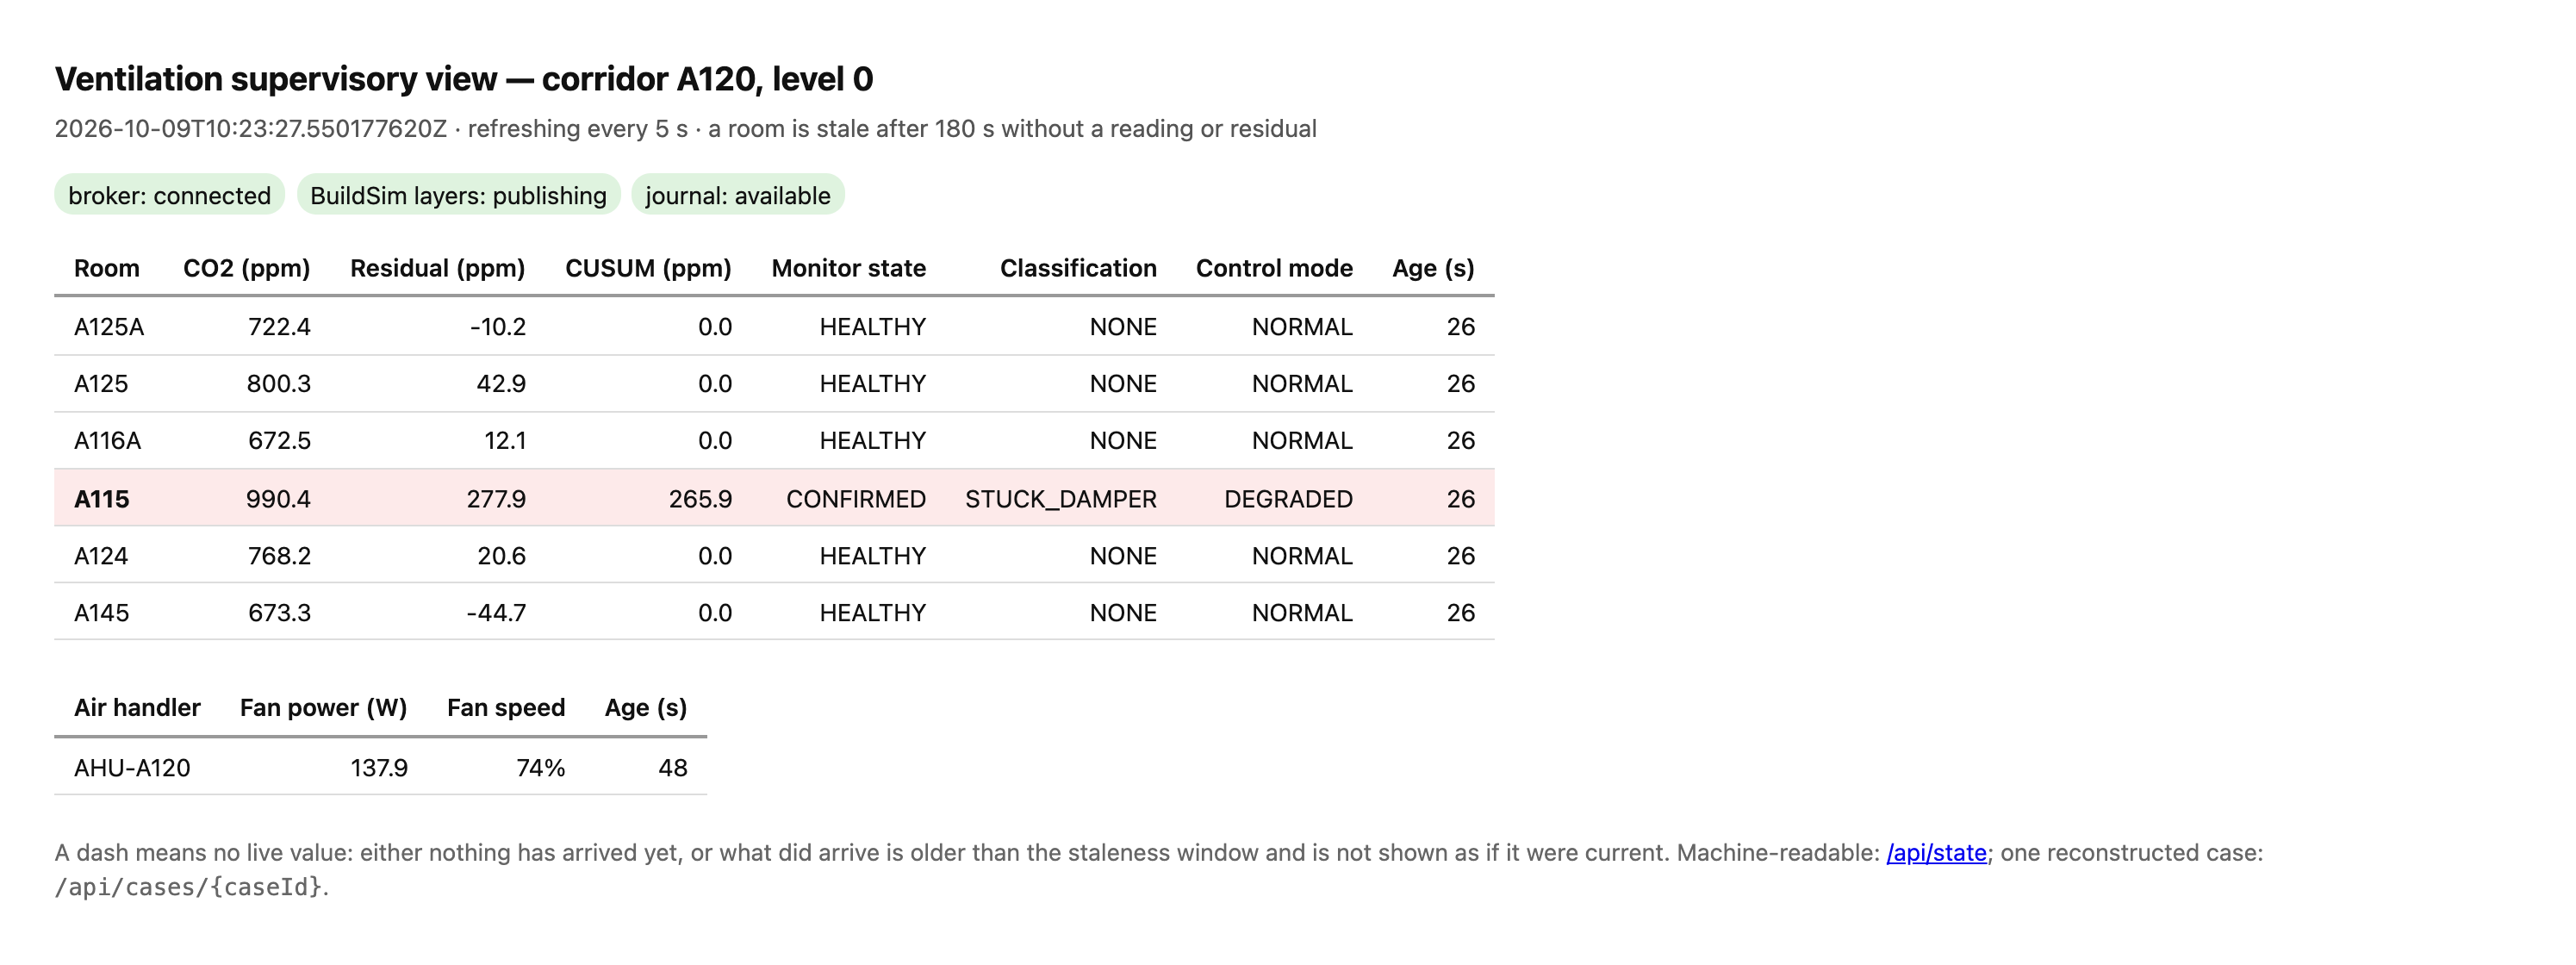
\includegraphics[width=\linewidth]{screenshots/dashboard-confirmed.png}
\caption{Simulated 10:23:27, the same run. A115's row is pink and bold: 990.4~ppm, residual
277.9~ppm, CUSUM 265.9~ppm, \texttt{CONFIRMED} / \texttt{STUCK\_DAMPER} / \texttt{DEGRADED}, with
the air handler at 137.9~W and 74~\%. The other five rooms are \texttt{HEALTHY} at CUSUM 0.0,
which is R-7's isolation visible in one frame. All three dependency pills are green, including
\texttt{BuildSim layers: publishing}.}
\end{figure}

\begin{figure}[!htbp]
\centering
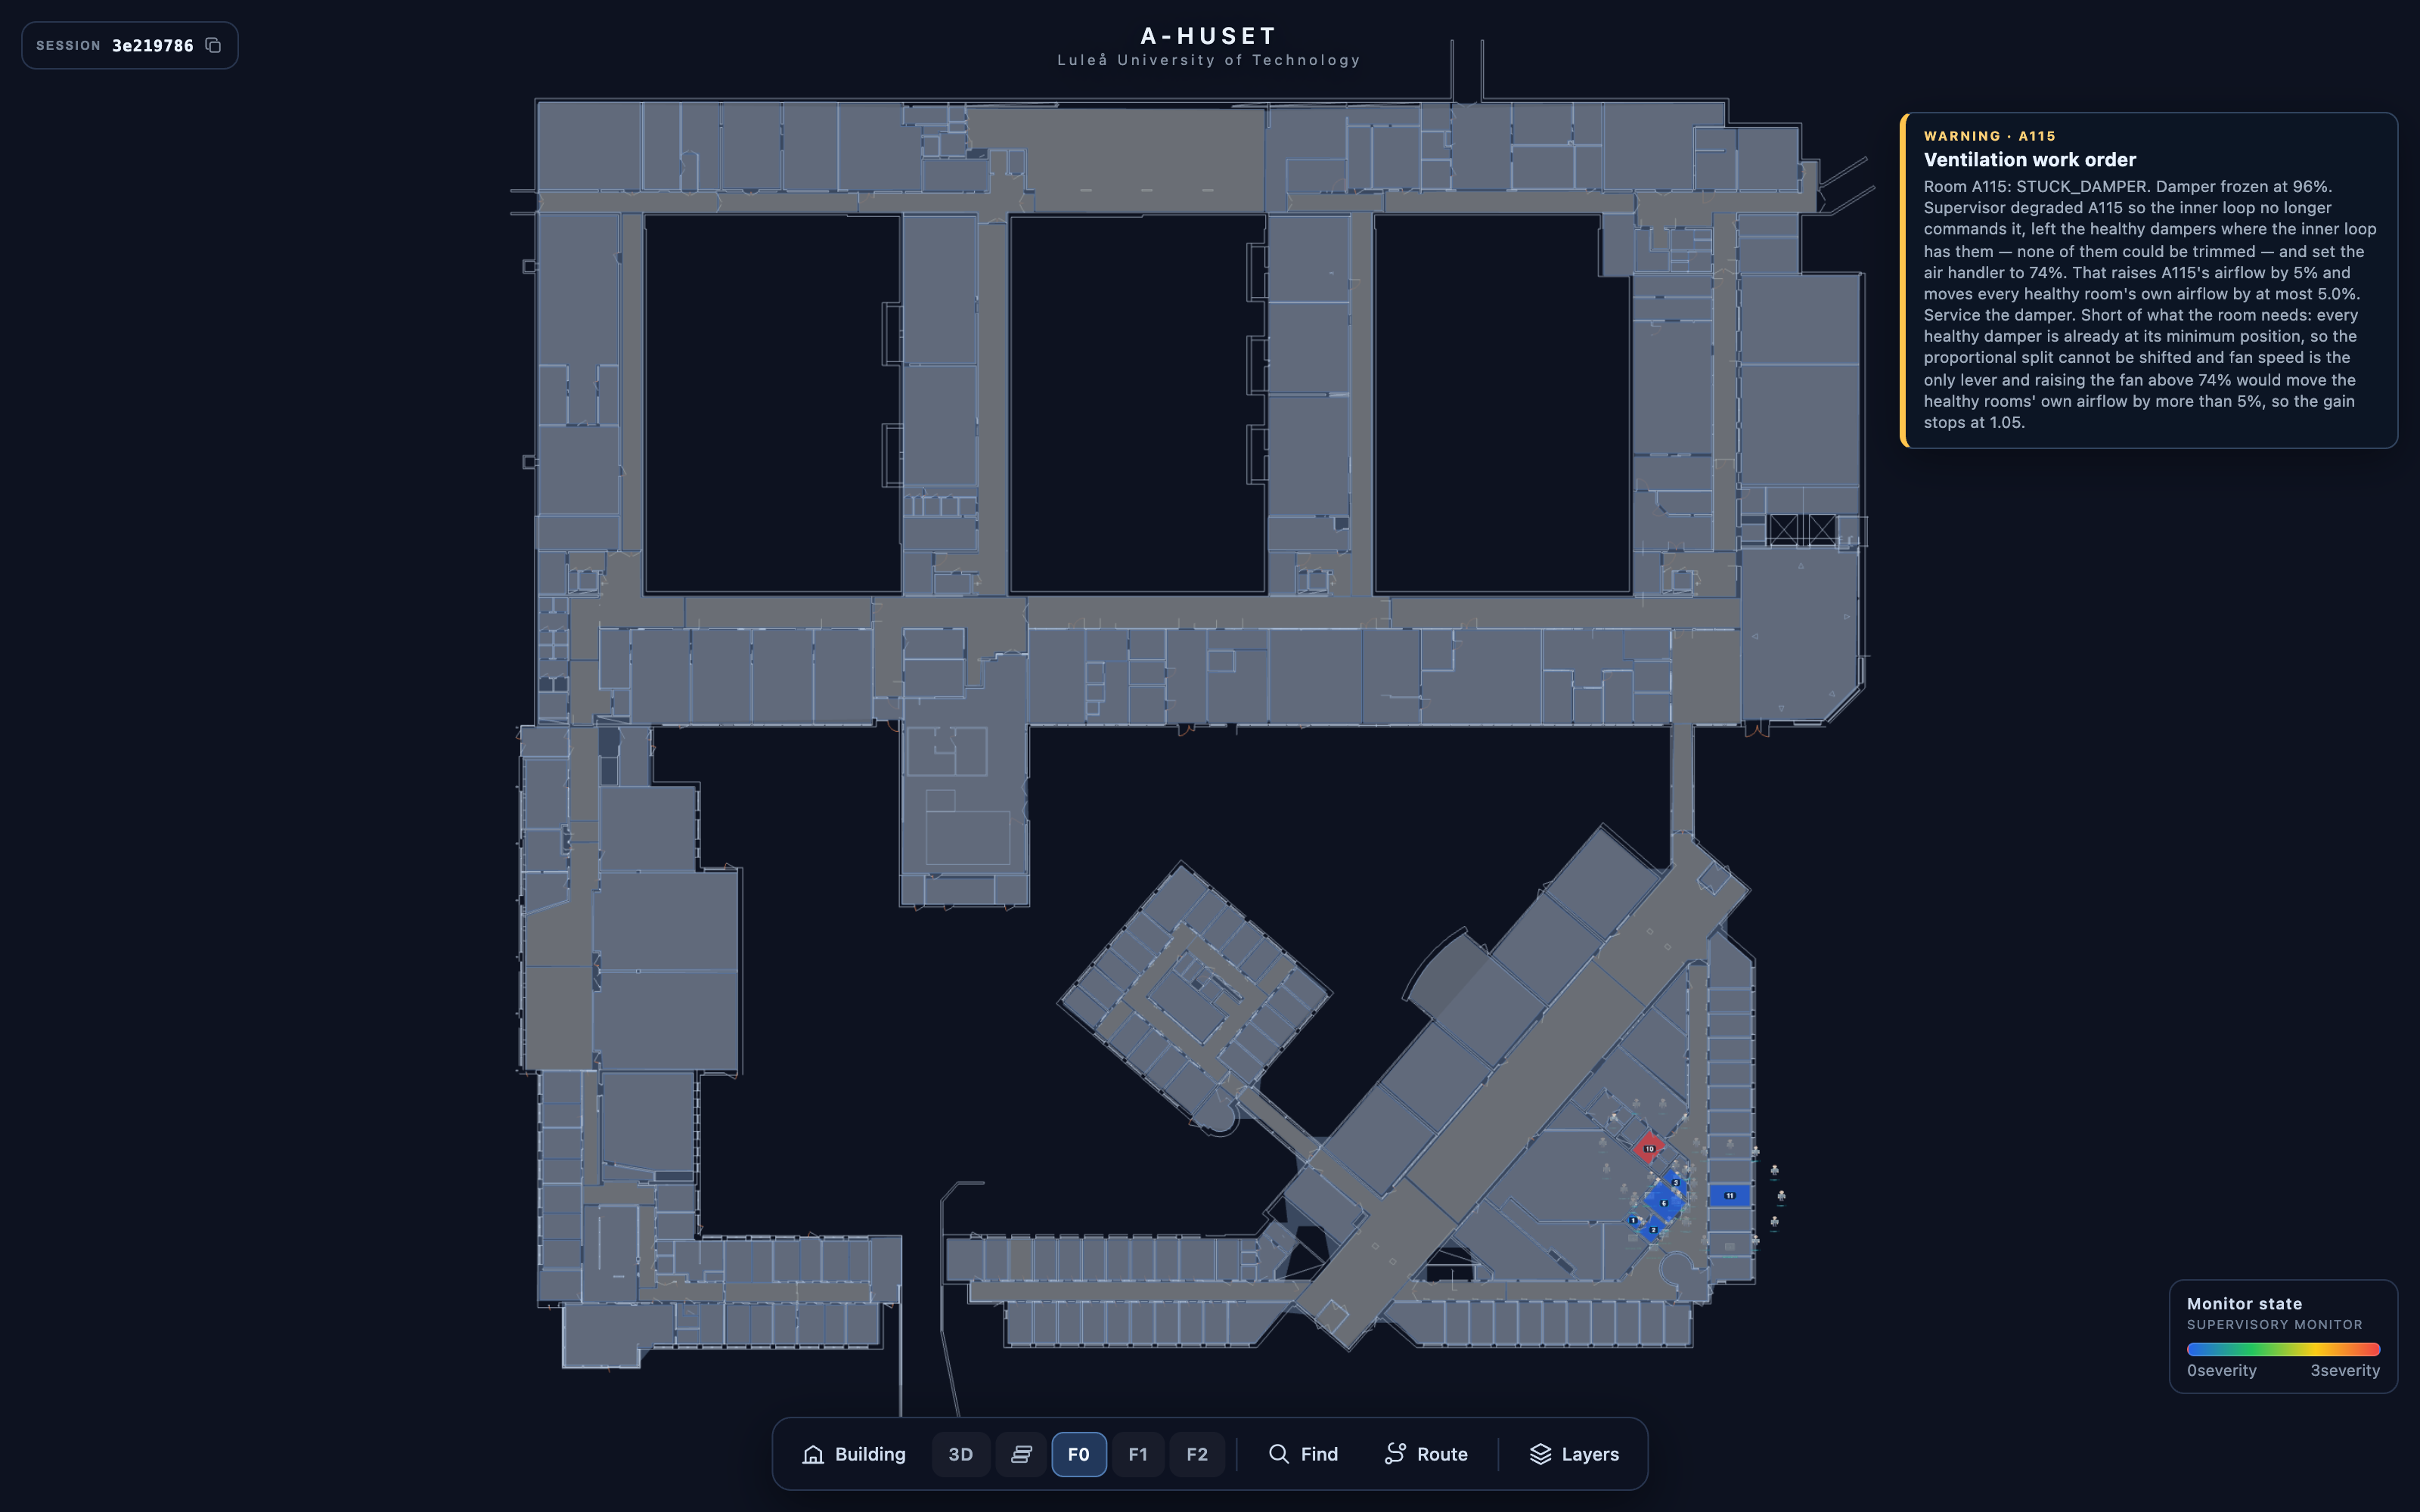
\includegraphics[width=\linewidth]{screenshots/buildsim-state-workorder.png}
\caption{The same instant on BuildSim's own floor plan, \texttt{?layer=state}. A115 is the single
hot room. The panel on the right is rendered by BuildSim from the alert the \emph{supervisor} PUT,
and it names the diagnosis, the action taken and the bound the plan ran into: the fan cannot be
raised above 74~\% without moving the healthy rooms' own airflow by more than 5~\%, so the gain
stops at 1.05. The legend at the lower right is the severity scale the \texttt{state} layer is
painted on.}
\end{figure}

\begin{figure}[htbp]
\centering
\begin{minipage}{0.48\linewidth}\centering
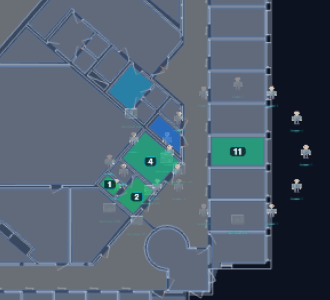
\includegraphics[width=\linewidth]{screenshots/buildsim-layer-co2.png}\\[2pt]
{\footnotesize\texttt{co2}: A115 at 562~ppm, second \emph{lowest} of the six}
\end{minipage}\hfill
\begin{minipage}{0.48\linewidth}\centering
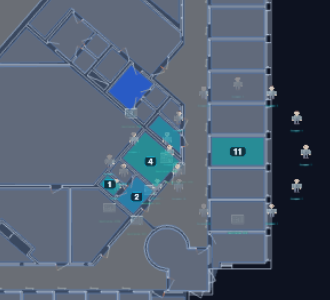
\includegraphics[width=\linewidth]{screenshots/buildsim-layer-residual.png}\\[2pt]
{\footnotesize\texttt{residual}: A115 at the scale floor, $-100$}
\end{minipage}

\vspace{6pt}
\begin{minipage}{0.48\linewidth}\centering
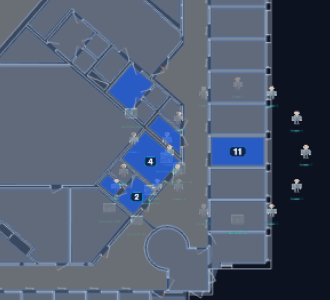
\includegraphics[width=\linewidth]{screenshots/buildsim-layer-cusum.png}\\[2pt]
{\footnotesize\texttt{cusum}: A115 at 0.0, like every other room}
\end{minipage}\hfill
\begin{minipage}{0.48\linewidth}\centering
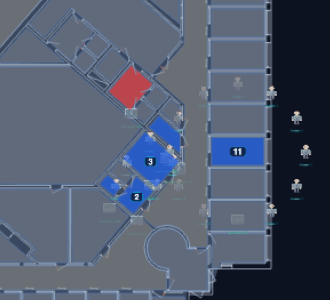
\includegraphics[width=\linewidth]{screenshots/buildsim-layer-state.png}\\[2pt]
{\footnotesize\texttt{state}: A115 at severity 3, the only non-zero room}
\end{minipage}
\caption{Corridor A120 painted by all four layers at one instant, simulated 11:40:55, with A115
latched and \texttt{COMPENSATING}. \textbf{This is the argument of Section \ref{sec:12}, measured rather than
asserted.} Compensation has done its job, so on \texttt{co2} the broken room is the second coolest
on the floor (562~ppm against its neighbours' 478--747), on \texttt{residual} it sits at the bottom
of the scale, and on \texttt{cusum} it is indistinguishable from five healthy rooms. Only
\texttt{state} still says the equipment is broken. \textbf{This figure could not be taken before
the room-layer defect below was fixed}, because three of these four layers never reached BuildSim.}
\end{figure}

% The four-layer frame is most of a page on its own, so it cannot follow the other two. This flushes
% it before H.2 begins rather than letting it land in the middle of H.2's prose.
\clearpage
\subsection{Two defects the capture found, and one limit it exposed}\label{sec:H.2}

\textbf{The layers were overwriting each other.} \texttt{/api/room-layers} is a collection
endpoint and a PUT replaces the whole collection, exactly as \texttt{/api/alerts} does, and the
dashboard was publishing its four layers one at a time, so each call erased the one before it.
Only the last layer of the enum, \texttt{state}, ever reached BuildSim; the other three selected
nothing. Every individual PUT returned 200, so nothing anywhere said so, and the adapter's own
work-order path had the collection semantics right the whole time two methods away. The fix is to
send every layer on every call, and the regression test drives a real HTTP stub rather than a mock,
because the defect was in what went over the wire. A mock of the adapter's own method would have
asserted the bug. The run above confirms it against the real stack and not only the stub:
\texttt{GET /api/room-layers} returns \textbf{four layers of six zones each}.

\textbf{A compensated room is painted exactly like a dead sensor.} At the instant of the four-layer
figure A115's true residual was $-303.9$~ppm. The \texttt{residual} layer's range starts at $-100$,
so \texttt{RoomLayer.onScale} clamps it to $-100$, and $-100$ is also the value that same method
returns for a \emph{stale} room, because the bottom of the scale is the only no-data encoding
BuildSim's layer API offers. On that layer a deeply compensated room and a room whose sensor has
died are therefore the same colour. The range itself is not the error: it was set from measured
healthy residuals spanning $-76.5$ to $+80.3$~ppm and a stuck damper's post-command mean of
507.8~ppm, and widening it to reach $-400$ would spend most of the scale on a regime the operator
almost never reads, making ordinary healthy variation invisible. So this is recorded as a limit
rather than patched: the dashboard table carries the true number one click away, and the
\texttt{state} layer already carries the fact that matters. It is also a limit that \emph{only
became observable} once the layers started arriving at all.

\textbf{\texttt{SUSPECT} cannot be photographed, and now that is measured.} A 1~Hz poll of
\texttt{/api/state} across the whole run caught A115 in \texttt{SUSPECT} in \textbf{2 of 295
usable samples} (296 polls were written and the last was truncated by the teardown), CUSUM 108.5 then 153.5~ppm, on residuals of 274.9 and 190.8~ppm, against a page
that refreshes every 5~s. A state that persists for two seconds may never be drawn at all, so it
is evidenced from the \texttt{decisions} journal and from the poller, and the screenshots are taken
only at states that latch. The instrument, not the intention, is what decides which evidence a
behaviour can carry.
